Una señal de sonido no es más que la variación en la presión que ejerce el medio que la transmite sobre su receptor.
La percepción del sonido en los seres humanos ocurre en dos regiones fundamentales: la \textit{periférica} y la \textit{nerviosa}.
Comienza en los oídos y continúa a través de la cóclea, en el oído interno, donde las variaciones en la presión del aire son transformadas en impulsos nerviosos conducidos hacia la corteza cerebral.

El hertz (Hz) es la unidad que expresa la cantidad de vibraciones que emite una fuente sonora en cada segundo de tiempo (frecuencia).
Se considera que el oído humano puede percibir ondas sonoras de frecuencias entre los 20 y los 20~000 Hz.

Un sonido puede ser representado de forma simple mediante un \textbf{oscilograma} (figura~\ref{img:oscillogram}), donde el eje X representa el tiempo, y el eje Y representa la \textit{amplitud} de la presión del sonido (generalmente usando unidades de media arbitrarias).

\begin{figure}[!h]
    \centering
    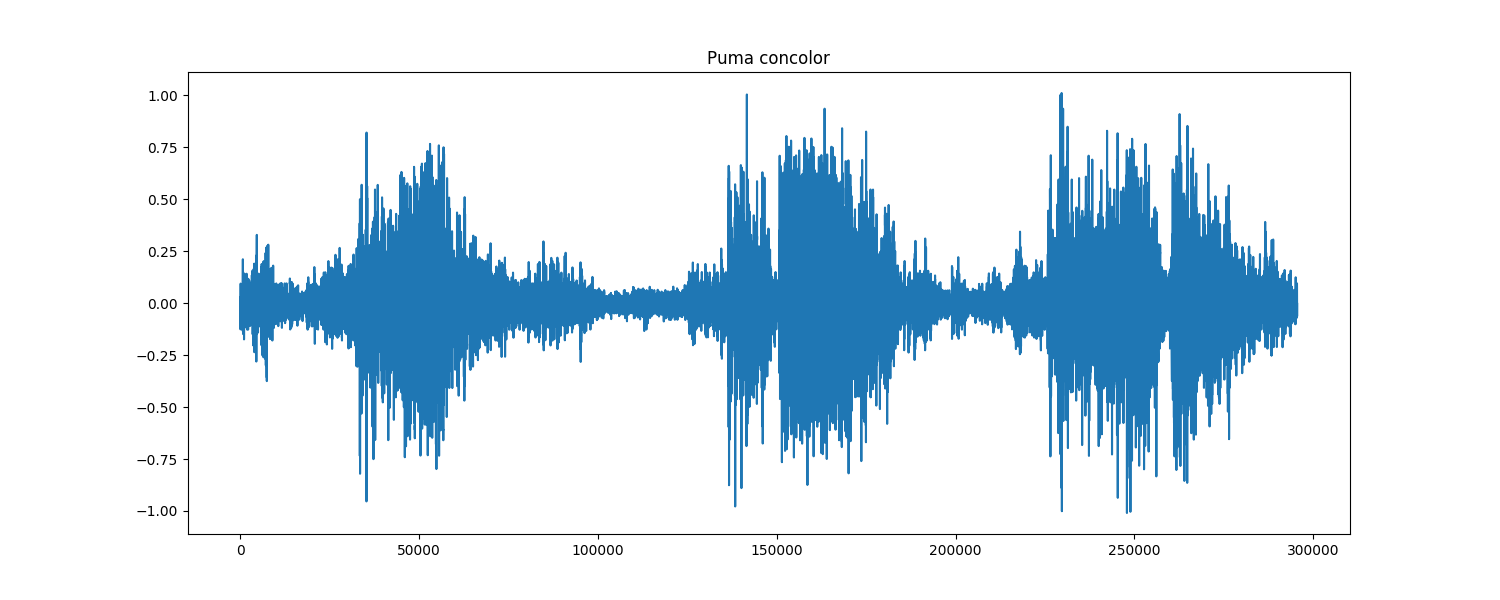
\includegraphics[width=\textwidth]{oscillogram.png}
    \caption{Oscilograma de una vocalización de un individuo de la especie \textit{puma concolor}.}
    \label{img:oscillogram}
\end{figure}

Una importante clase de sonidos son aquellos que consisten en oscilaciones que se repiten periódicamente cada un cierto tiempo.
La duración de una de estas oscilaciones es conocida como su \textit{período} (en segundos) y a la medida inversa se le denomina \textit{frecuencia} (en Hz).
Existen otros sonidos de características aleatorias y que no se repiten periódicamente, llamados \textit{ruidos}.

Una oscilación puede ser descompuesta en una suma de sinusoides elementales de diferentes frecuencias, mediante la aplicación de la \textbf{transformada de Fourier}.
La representación de la transformada de Fourier de una señal en un tiempo dado es conocida como su \textbf{espectro} (figura~\ref{img:spectrum+spectrogram}a).
Esta transformada puede ser igualmente computada sobre pequeñas ventanas de tiempo superpuestas, lo que produce una representación tridimensional de la intensidad de las frecuencias en el tiempo, que llamamos \textbf{espectrograma} (figura~\ref{img:spectrum+spectrogram}b).

\begin{figure}[!h]
    \centering
    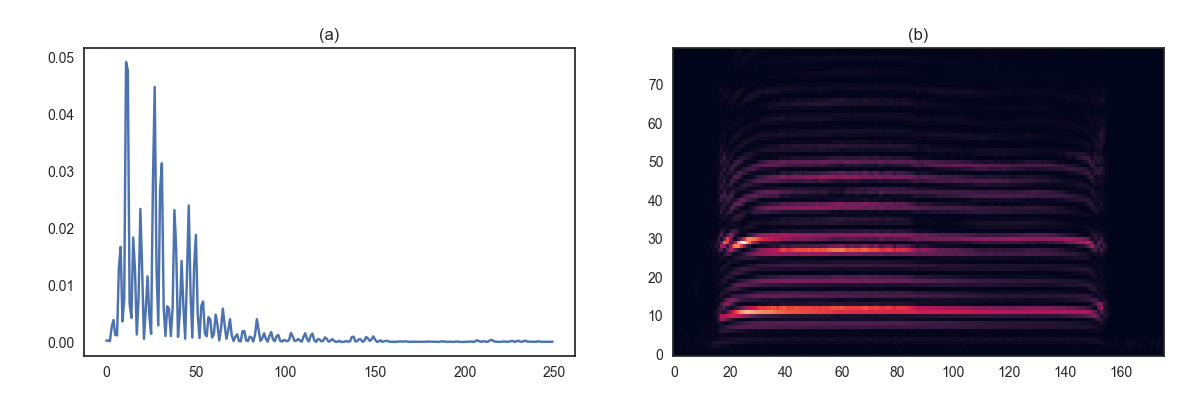
\includegraphics[width=\textwidth]{spectrum+spectrogram.png}
    \caption{Representaciones de la transformada de Fourier de la señal de la figura~\ref{img:oscillogram}: (a) Espectro del segundo 2. (b) Espectrograma.}
    \label{img:spectrum+spectrogram}
\end{figure}

Para el procesamiento computacional de una señal, esta debe ser llevada del dominio analógico al digital, para lo cual se discretiza mediante observaciones realizadas a intervalos regulares.
Los pasos más importantes en esta conversión de la señal de analógica a digital son:

\begin{enumerate}
    \item \textbf{Filtrado}: La señal analógica se filtra con el propósito de limitar las frecuencias presentes al intervalo $[0,B]$, donde $B$ es la frecuencia \textit{máxima} o \textit{de corte}.
    \item \textbf{Muestreo}: Se digitaliza la señal resultante del paso anterior;
    se emplea \textit{frecuencia de muestreo} $F_s = 2B$ para evita el fenómeno de \textit{aliasing}\footnote{Efecto que causa que señales continuas distintas se tornen indistinguibles cuando se muestrean digitalmente.
    Cuando esto sucede, la señal original no puede ser reconstruida de forma unívoca a partir de la señal digital.}.
    \item \textbf{Cuantificación}: La señal digital es cuantificada, se limita el espacio de almacenamiento ocupado por cada muestra.
\end{enumerate}

Para una calidad de audio de CD se emplean valores de muestreo $F_s = 44.1$ kHz y una cuantificación de 16 bits por muestra.

Los algoritmos de inteligencia artificial tradicionalmente operan con vectores numéricos, llamados \textit{vectores de características}.
En las siguientes secciones analizamos los procedimientos mediante los cuales una señal de audio digital se transforma en una secuencia de tales vectores.

\section{Ventanas}\label{sec:frames}

Para procesar una señal esta a menudo es dividida en pequeños segmentos, conocidos como \textit{ventanas}\footnote{\textit{frames} en inglés.}, de longitud constante y espaciados en intervalos de tiempo iguales.
Denotamos por $N$ la cantidad de muestras de la señal que contiene una ventana;
de esta forma la duración de una ventana será de $N/F_s$.
Asimismo, denotamos por $M$ la cantidad de muestras en que difieren dos ventanas consecutivas, conocida como \textit{tamaño de paso}, y que usualmente es menor que $N$.
A partir de estos valores podemos igualmente calcular la cantidad de muestras que dos ventanas consecutivas tienen en común, como $N-M$;
y el número de ventanas por segundo (\textit{frame rate}) como $F_s/M$.

Cada ventana de $N$ muestras es usualmente obtenida mediante la aplicación de una función $w(t)$ a la señal, que es distinta de cero solo si $1\leq t\leq N$.
Dada la señal $s(t)$, una ventana que comienza en la muestra $m$ es obtenida como

\begin{equation}
    \label{eq:windowing}
    s(t)_m = \begin{cases}
                 s(t + m-1)w(t) & 1\leq t\leq N \\
                 0 & eoc.
    \end{cases}
\end{equation}

Existen diferentes variantes muy empleadas para la función $w(t)$.
Dos de ellas son las siguientes:

\begin{itemize}
    \item \textbf{Rectangular}:
    \[
        w(t) = \begin{cases}
                   1 & 1\leq t\leq N \\
                   0 & eoc.
        \end{cases}
    \]
    \item \textbf{Hamming}:
    \[
        w(t) = 0.53836 - 0.46164 \cos\left(\frac{2\pi t}{N-1}\right)
    \]
\end{itemize}

La elección de la función $w(t)$ tiene un efecto sobre los resultados de operaciones posteriores sobre las ventanas obtenidas.
En la práctica, algunos métodos de procesamiento, como la transformada de Fourier producen mejores resultados cuando se emplean funciones que se aproximan a cero en sus extremos, como la de Hamming.
